\section{Manuale utente}
\subsection{Prerequisiti}
Il programma pu\`{o} essere eseguito solo su macchine Unix-like. Inoltre, per la compilazione,
\`{e} necessario disporre delle seguenti componenti:
\begin{itemize}
\item gnatmake 4.4.3
\item gcc 4.4.3
\item librerie \textbf{XmlAda 3.2w} installate con comando \underline{xmlada-config} eseguibile anche senza privilegi di root.\\
In caso contrario, scaricare il pacchetto XMLAda da\\
\url{http://libre.adacore.com/libre/download2/}\\
e, dopo la decompressione, seguire le istruzioni incluse per la compilazione ed installazione.
\item librerie \textbf{PolyORB GPL 2009-20090519 (rev. 144248)} installate con comando \underline{polyorb-config} eseguibile anche 
senza privilegi di root\\
In caso contrario, scaricare il pacchetto PolyORB da\\
\url{http://libre.adacore.com/libre/download2/}\\
e, dopo la decompressione, seguire le istruzioni incluse per la compilazione ed installazione.
\end{itemize}
La versione indicata delle librerie \`{e} quella usata per i test. Non si esclude tuttavia che il programma possa funzionare anche con versioni
appena precedenti o successive.
\subsection{Installazione}
Dalla directory radice, eseguire i seguenti comandi:
\begin{itemize}
\item \emph{make competition}\\
per compilare la componente destinata a ospitare la competizione
\item \emph{make box}\\
per compilare la componente destinata a eseguire il box
\item \emph{make tv}
per compilare la componente che verr\`{a} usata per la TV
\end{itemize}
Le tre componenti hanno make diversi perch\`{e} possono essere compilate ed eseguite su macchine separate, comunicando remotamente.
\subsection{Avvio}
Come per la compilazione, dalla directory radice esecuire il comando desiderato fra i seguenti:
\begin{itemize}
\item \emph{./start\_competition.sh}\\
avvier\`{a} la competizione. Apparir\`{a} il pannello di configurazione (del quale verranno forniti dettagli in seguito)
\item \emph{./start\_box.sh n}\\
avvier\`{a} un numero n box. Per eseguire un test in locare \`{e} possibile avviare tanti box quanti quelli stabiliti durante la configurazione
della competizione. In tal caso, l'interfaccia di configurazione dei box presenter\`{a} nello spazio riservato al corbaloc per la connessione
alla competizione, il corbaloc della competizione caricato dal contesto locale.
\item \emph{./start\_tv.sh}\\
inizializza una tv. Anche in questo caso, se il corbaloc della competizione \`{e} presente in locale, verr\`{a} impostato di default nel textbox
dedicato. \`{E} comunque possibile reimpostarlo.
\end{itemize}
L'interfaccia TV \`{e} possibile copiarla senza necessit\`{a} di ricompilazione in tutte le macchine ove la si voglia eseguire. E' sufficiente,
una volta compilata, copiare il file \emph{start\_tv.sh} e la directory \emph{obj/java/GUI} (mantenendo la gerarchia intatta) in un qualunque
nodo distribuito ed eseguire lo starter.
\subsection{Terminazione}
Per terminare il programma (box, competizione o tv che sia) premere il tasto ``x'' in alto a destra sulla finestra.
\subsection{Interfaccia box}
Nella prima schermata che appare vanno inseriti i dati relativi al concorrente che si intende registrare.
\begin{enumerate}
\item Impostare il nome del concorrente
\item Impostare il cognome del concorrente
\item Impostare la scuderia del concorrente
\item Impostare il livello di seriet\`{a} del box (come descritto da \ref{box})
\item Impostare la massima capacit\`{a} del serbatoio
\item Impostare il livello di benzina iniziale
\item Impostare la mescola delle gomme montate (le gomme a mescola morbida si consumano pi\`{u} rapidamente)
\item Impostare lo stile di guida del concorrente 
\item Impostare la massima accelerazione della macchina
\item Impostare la massima velocit\`{a} raggiungibile
\item Inserire il corbaloc che fa riferimento al Registration Hanlder
\item Pulsante per avviare la competizione
\item Pulsante per riportare la gui allo stato iniziale
\end{enumerate}
\begin{center}
\begin{figure}[H]
	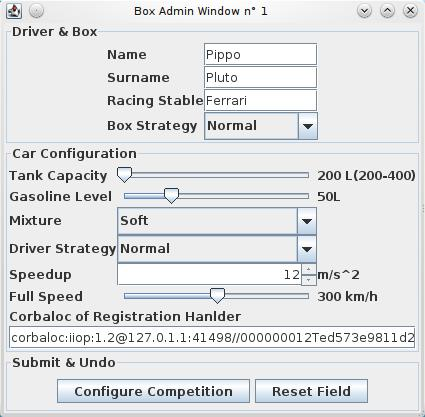
\includegraphics[scale=0.75]{img/ScreenshotRelazione/BoxAdminWindows.jpg}
	\caption{Finestra di configurazione del box e del concorrente}
\end{figure}
\end{center}
Una volta inseriti i dati e premuto il pulsante di avvio della competizione comparir\`{a} una finestra con al suo interno 
\begin{enumerate}
\item Pannello dei consumi medi del concorrente con dati relativi alla benzina (in litri al kilometro) e dell'usura delle gomme (in percentuale relativo a 1 km)
\item Pannello con il log della gara aggiornato a ogni fine settore con dati di tempo di gara, livello di benzina e usura delle gomme
\item Pannello con altre informazioni statiche sulla gara (configurazione iniziale, stile di guida)
\end{enumerate}
\begin{center}
\begin{figure}[H]
	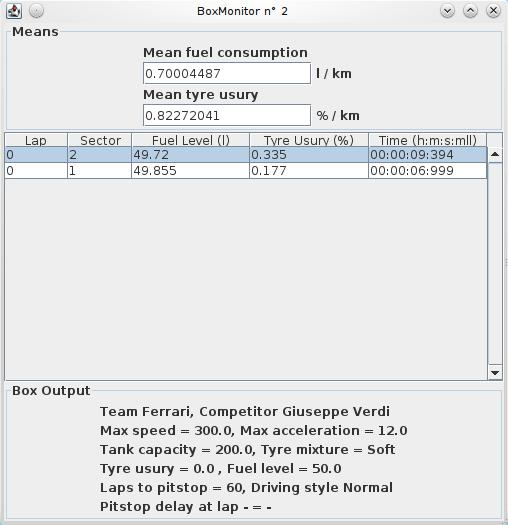
\includegraphics[scale=0.75]{img/ScreenshotRelazione/boxMonitor.jpg}
	\caption{Monitor dei box}
\end{figure}
\end{center}
\subsection{Interfaccia competizione}
La prima interfaccia relativa alla competizione serve per impostare la competizione stessa. I parametri da settare sono:
\begin{enumerate}
\item File xml con il tracciato\\
il formato per il file xml del tracciato \`{e} il seguente:
\begin{lstlisting}
<racetrack>
  <sector>
      <checkpoint>
	<length>19.00</length>
	  <mult>7</mult>
	  <angle>140.00</angle>
	  <grip>7.0</grip>
      </checkpoint>
      <!-- altri checkpoint-->
  </sector>
  <!--altri 3 sector strutturati allo stesso modo-->
</racetrack>
\end{lstlisting}
Il checkpoint pu\`{o} avere uno dei seguenti attributi:
\begin{itemize}
\item \textbf{goal=``true''}: obbligatorio in massimo 1 checkpoint. Indica il checkpoint di partenza.
\item \textbf{prebox=``true''}: obbligatorio in massimo 1 checkpoint nel settore 3.
\item \textbf{exitbox=``true''}: obbligatorio in massimo 1 checkpoint nel settore 1.
\end{itemize}
\item Numero di concorrenti richiesti
\item Numero di giri previsti
\item Nome del tracciato
\end{enumerate}
Una volta settati i parameteri e schiacciato il pulsante \emph{Start Competition} verr\`{a} avviato una tv che presenta le informazioni sulle iscrizioni nella parte bassa della finestra. Ogni volta che un concorrente si iscrive compare nella gui e una volta raggiunto il numero di concorrenti stabiliti la gara si avvia e la gui comincia ad offrire i dati disponibili, come spiegato nel paragrafo \ref{interfacciaTv}
\begin{center}
\begin{figure}[H]
	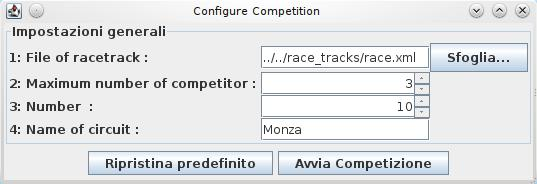
\includegraphics[scale=0.75]{img/ScreenshotRelazione/configureCompetition.jpg}
	\caption{Finestra di configurazione della competizione}
\end{figure}
\end{center}
\subsection{Interfaccia TV}
\label{interfacciaTv}
L'interfaccia della tv consiste in un pannello iniziale con al suo interno un cronometro che scandisce il tempo di aggiornamento delle informazioni seguito da un pannello con le informazioni sul miglior giro e sui migliori tempi nei settori.
L'intervallo per il tempo che scorre \`{e} impostabile se si tratta di una tv configurata tramite il \emph{TvConfigurationWindow}, prestabilito (e molto basso) se si tratta della tv avviata dalla competizione. Il formato della stringa di refresh dev'essere \emph{secondi . millisecondi}.
Il pannello centrale offre la visualizzazione di due tabelle. La tabella a destra si riferisce all'ultima classifica disponibile mentre a sinistra viene visualizzata la classifica del giro precedente (escluso al primo giro di gara dove viene presentata una tabella vuota).
Nella parte bassa della finestra viene presentato un log della competizione rappresentando a ogni istante di tempo posizione nella pista, numero di checkpoint, numero di settore e giro per ogni concorrente.
\begin{center}
\begin{figure}[h]
	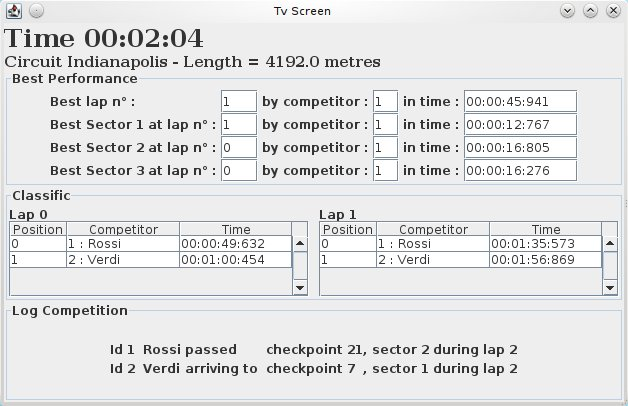
\includegraphics[scale=0.75]{img/ScreenshotRelazione/screenTvCompetition.jpg}
	\caption{Finestra di visualizzazione dell'andamento della gara}
\end{figure}
\end{center}
La componente di avvio dell'interfaccia TV pu\`{o} essere l'interfaccia di competizione oppure una schermata di configurazione dove va inserito il corbaloc del Monitor della competizione e impostato il tempo di refresh per il reperimento delle informazioni.
\begin{center}
\begin{figure}[H]
	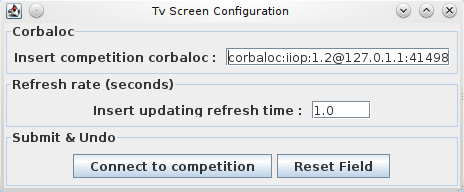
\includegraphics[scale=0.75]{img/ScreenshotRelazione/configurationScreen.jpg}
	\caption{Finestra di configurazione della tv}
\end{figure}
\end{center}